% ===========================================================
%  Chapter 9 — Actor-Critic Methods and Proximal Policy Optimization
% ===========================================================
\chapter[Actor-Critic Methods and PPO]{Actor-Critic Methods and Proximal Policy Optimization}
\label{ch:actor-critic}

\begin{quote}
\itshape
The idea of having two interacting components, one for behavior and one for
criticism, seems to be as old as the idea of reinforcement learning itself.
\upshape\hfill---Richard S.\ Sutton and Andrew G.\ Barto, \textit{Reinforcement Learning: An Introduction}
\end{quote}

\bigskip

Chapter~\ref{ch:pg} developed the policy gradient theorem and the REINFORCE
algorithm, establishing that one can directly optimize a parameterized policy
by following the gradient of the expected return.  REINFORCE is
conceptually elegant but suffers from a fundamental statistical weakness: its
gradient estimator uses the full discounted return $G_t$ as a signal for
every action taken in an episode.  Because $G_t$ is a sum of many random
rewards stretching to the end of the episode, its variance grows with the
horizon, leading to slow and noisy learning.

The remedy introduced in this chapter is to replace $G_t$ with a lower-variance
estimate of how much better than average a particular action was\,---\,the
\emph{advantage function}\,---\,and to learn this estimate online using a
second neural network called the \emph{critic}.  The resulting class of
algorithms is known as \textbf{actor-critic} methods.
\index{actor-critic}
The actor (the policy) and the critic (the value function) interact on every
time step: the critic evaluates the actor's choices, and the actor uses that
evaluation to update its parameters.

From this foundation we build progressively more powerful algorithms.
Generalized Advantage Estimation (GAE) provides a flexible bias-variance
tradeoff for the advantage signal.  Asynchronous Advantage Actor-Critic (A3C)
exploits parallel workers to decorrelate experience and accelerate training.
Trust Region Policy Optimization (TRPO) introduces the key insight that policy
updates must be constrained to remain close to the current policy.  Proximal
Policy Optimization (PPO) achieves the same effect with a simple clipping
mechanism that is fast, easy to implement, and remarkably robust in practice.
Finally, we study how PPO is deployed for fine-tuning large language models
with human feedback, the paradigm known as RLHF.

% -----------------------------------------------------------
\section{The Advantage Function}
\label{sec:advantage}
% -----------------------------------------------------------

\subsection{Definition and Basic Properties}

Recall from Chapter~\ref{ch:pg} that the policy gradient theorem
expresses the gradient of the objective in terms of the action-value function:
\begin{equation}
\label{eq:pg-theorem-repeat}
\nabla_\theta J(\theta)
= \E_{S \sim d^\gamma_{\pi_\theta},\; A \sim \pi_\theta(\cdot|S)}
  \bigl[\nabla_\theta \log \pi_\theta(A \mid S)\; Q^{\pi_\theta}(S, A)\bigr].
\end{equation}
Chapter~\ref{ch:pg} also showed that any \emph{state-dependent} baseline
$b(S_t)$ can be subtracted from $Q^{\pi_\theta}(S_t, A_t)$ without
changing the expected gradient (Proposition~8.2 in Chapter~\ref{ch:pg}).
The best possible baseline is the one that most reduces variance, and
under mild conditions the optimal choice is precisely the state-value function
$V^{\pi_\theta}(s)$.  The difference that remains after subtracting this
baseline is so important that it deserves its own name.

\begin{definition}[Advantage function]
\label{def:advantage}
\index{advantage function}
For a policy $\pi$ and the induced action-value and state-value functions
$Q^\pi$ and $V^\pi$, the \textbf{advantage function} is
\begin{equation}
\label{eq:advantage-def}
A^\pi(s, a) \;=\; Q^\pi(s, a) - V^\pi(s).
\end{equation}
\end{definition}

Intuitively, $A^\pi(s,a)$ measures the relative quality of action $a$ compared
with the average action the policy would take in state $s$.  A positive
advantage means that $a$ is better than average; a negative advantage means
it is worse.  This centring property is formalized in the following proposition.

\begin{proposition}[Zero-mean advantage]
\label{prop:advantage-zero-mean}
\index{advantage function!zero-mean property}
For any policy $\pi$ and any state $s \in \cS$,
\begin{equation}
\label{eq:advantage-zero-mean}
\E_{A \sim \pi(\cdot|s)}\bigl[A^\pi(s, A)\bigr] = 0.
\end{equation}
\end{proposition}

\begin{proof}
By Definition~\ref{def:advantage} and linearity of expectation,
\[
\E_{A \sim \pi(\cdot|s)}\bigl[A^\pi(s, A)\bigr]
= \E_{A \sim \pi(\cdot|s)}\bigl[Q^\pi(s, A)\bigr] - V^\pi(s).
\]
The Bellman equation (Chapter~\ref{ch:mdp}, Equation~(3.12)) gives
$V^\pi(s) = \sum_a \pi(a|s)\,Q^\pi(s,a)
           = \E_{A \sim \pi(\cdot|s)}[Q^\pi(s,A)]$,
so the right-hand side is zero.
\end{proof}

Substituting $V^{\pi_\theta}(S_t)$ for the baseline in the policy gradient
formula~\eqref{eq:pg-theorem-repeat} yields the \textbf{advantage form} of
the policy gradient:
\begin{equation}
\label{eq:advantage-pg}
\nabla_\theta J(\theta)
= \E_{S \sim d^\gamma_{\pi_\theta},\; A \sim \pi_\theta(\cdot|S)}
  \bigl[\nabla_\theta \log \pi_\theta(A \mid S)\; A^{\pi_\theta}(S, A)\bigr].
\end{equation}
This is the version of the policy gradient theorem that underlies all
actor-critic algorithms.

\subsection{Why the Advantage Reduces Variance}

To see concretely why using $A^\pi(s,a)$ instead of $Q^\pi(s,a)$ helps,
consider a simple example.

\begin{example}[Advantage versus raw return]
\label{ex:advantage-variance}
Suppose an agent is in state $s$ where every action yields a high return
because $s$ is already a very good state.  Concretely, assume
$Q^\pi(s, a) \in \{8, 10, 12\}$ with equal probability for three actions,
so $V^\pi(s) = 10$.  The raw action-value scores have mean 10 and variance
$\Var[Q^\pi(s,\cdot)] = \frac{4+0+4}{3} \approx 2.67$.

The advantage scores are $A^\pi(s,a) \in \{-2, 0, 2\}$, which have mean 0
(consistent with Proposition~\ref{prop:advantage-zero-mean}) and the same
variance 2.67.  At first glance the variance is unchanged, but notice the
crucial difference: because the policy gradient update is
$\nabla_\theta \log \pi_\theta(a|s) \cdot A^\pi(s,a)$, updates for the
mediocre action ($A = 0$) are zero regardless of the policy parameters.
Using the raw $Q$ would produce a nonzero gradient signal of magnitude 10
even for the neutral action, polluting the update with a large global
offset that must be cancelled across many samples.  The advantage removes
this offset perfectly and in expectation.\qed
\end{example}

More formally, the variance of the policy gradient estimator with the
optimal baseline $b^*(s)$ can be shown to satisfy
\begin{equation}
\label{eq:variance-reduction}
\Var\!\bigl[\nabla_\theta \log\pi_\theta(A|S)\,(Q^\pi(S,A) - b^*(S))\bigr]
\;\leq\;
\Var\!\bigl[\nabla_\theta \log\pi_\theta(A|S)\,Q^\pi(S,A)\bigr],
\end{equation}
and the reduction can be dramatic in environments where the value function
varies substantially across states but the advantage variation within each
state is modest.

% -----------------------------------------------------------
\section{The Actor-Critic Architecture}
\label{sec:actor-critic-arch}
% -----------------------------------------------------------

\subsection{Two-Component Design}

An actor-critic algorithm maintains two interacting components.

\begin{definition}[Actor and critic]
\label{def:actor-critic}
\index{actor}\index{critic}
An \textbf{actor-critic} algorithm maintains:
\begin{itemize}[leftmargin=*]
  \item an \textbf{actor}: a parameterized policy $\pi_\theta(a \mid s)$ whose
    parameters $\theta$ are updated to maximize $J(\theta)$;
  \item a \textbf{critic}: a parameterized value function $V_\phi(s)$ whose
    parameters $\phi$ are updated to approximate $V^{\pi_\theta}(s)$.
\end{itemize}
\end{definition}

The name reflects the metaphor of a performer (the actor) and a reviewer
(the critic): after every action, the critic signals whether that action
was above or below average, and the actor adjusts accordingly.

Figure~\ref{fig:actor-critic-diagram} illustrates the information flow.
The environment emits a state $S_t$; the actor selects action $A_t$; the
environment transitions to $S_{t+1}$ and emits reward $R_{t+1}$.  The
critic uses $(S_t, R_{t+1}, S_{t+1})$ to compute a TD error $\delta_t$,
which serves simultaneously as the critic's learning signal (it measures
how wrong the critic's own prediction was) and as an estimate of the
advantage to guide the actor's update.


\begin{figure}[ht]
\centering
\begin{tikzpicture}[
    node distance=1.8cm and 2.8cm,
    box/.style={rectangle, draw, rounded corners=4pt, minimum width=2.4cm,
                minimum height=0.9cm, font=\small, fill=blue!8},
    env/.style={rectangle, draw, rounded corners=4pt, minimum width=2.4cm,
                minimum height=0.9cm, font=\small, fill=orange!12},
    arr/.style={-Stealth, thick},
    lab/.style={font=\footnotesize, inner sep=2pt}
  ]

  % Layout
  \node[box]  (actor)  at (0,0)    {Actor $\pi_\theta$};
  \node[env]  (env)    at (5.5,0)  {Environment};
  \node[box]  (critic) at (0,-2.5) {Critic $V_\phi$};

  % Actor -> Env: action A_t
  \draw[arr] ([yshift=-4pt]actor.east) -- ([yshift=-4pt]env.west)
        node[lab, below, midway] {action $A_t$};

  % Env -> Actor: state S_t
  \draw[arr] ([yshift=4pt]env.west) -- ([yshift=4pt]actor.east)
        node[lab, above, midway] {state $S_t$};

  % Env -> Critic: reward + next state
  \draw[arr] (env.south) -- ++(0,-2.05) -- (critic.east)
        node[lab, above, pos=0.75] {$R_{t+1},\,S_{t+1}$};

  % Critic -> Actor: delta_t
  \draw[arr] (critic.north) -- (actor.south)
        node[lab, right, midway] {$\delta_t\!\approx\!\hat{A}_t$};

  % Annotation labels
  \node[lab, below=0.15cm of critic, text=blue!60!black] {\textit{learns $V^{\pi_\theta}$}};
  \node[lab, above=0.15cm of actor, text=blue!60!black]  {\textit{learns $\pi^*$}};

\end{tikzpicture}
\caption{Information flow in an actor-critic algorithm.  The actor selects
actions; the environment returns rewards and next states; the critic produces
a TD error $\delta_t$ that guides both critic and actor updates.}
\label{fig:actor-critic-diagram}
\end{figure}
% \begin{figure}[ht]
% \centering
% \begin{tikzpicture}[
%     node distance=1.8cm and 2.8cm,
%     box/.style={rectangle, draw, rounded corners=4pt, minimum width=2.4cm,
%                 minimum height=0.9cm, font=\small, fill=blue!8},
%     env/.style={rectangle, draw, rounded corners=4pt, minimum width=2.4cm,
%                 minimum height=0.9cm, font=\small, fill=orange!12},
%     arr/.style={-Stealth, thick},
%     lab/.style={font=\footnotesize, inner sep=2pt}
%   ]

%   % Layout: Actor top-left, Environment top-right, Critic bottom-left
%   \node[box]  (actor)  {Actor $\pi_\theta$};
%   \node[env]  (env)    [right=2.8cm of actor] {Environment};
%   \node[box]  (critic) [below=1.8cm of actor] {Critic $V_\phi$};

%   % Actor -> Env: action A_t  (runs below the midline to separate from return arrow)
%   \draw[arr] ([yshift=-4pt]actor.east) -- ([yshift=-4pt]env.west)
%         node[lab, below, midway] {action $A_t$};

%   % Env -> Actor: state S_t  (runs above the midline)
%   \draw[arr] ([yshift=4pt]env.west) -- ([yshift=4pt]actor.east)
%         node[lab, above, midway] {state $S_t$};

%   % Env -> Critic: reward + next state (straight line from env bottom to critic right)
%   \draw[arr] (env.south) -- ++(0,-0.6) -| (critic.east)
%         node[lab, below right, pos=0.3] {$R_{t+1},\,S_{t+1}$};

%   % Critic -> Actor: delta_t (advantage estimate)
%   \draw[arr] (critic.north) -- (actor.south)
%         node[lab, right, midway] {$\delta_t\!\approx\!\hat{A}_t$};

%   % Annotation labels
%   \node[lab, below=0.15cm of critic, text=blue!60!black] {\textit{learns $V^{\pi_\theta}$}};
%   \node[lab, above=0.15cm of actor, text=blue!60!black]  {\textit{learns $\pi^*$}};

% \end{tikzpicture}
% \caption{Information flow in an actor-critic algorithm.  The actor selects
% actions; the environment returns rewards and next states; the critic produces
% a TD error $\delta_t$ that guides both critic and actor updates.}
% \label{fig:actor-critic-diagram}
% \end{figure}

\subsection{Shared versus Separate Networks}

In practice, the actor and critic can be implemented in two ways.
When they are \textbf{separate networks}, the actor $\pi_\theta$ and critic
$V_\phi$ have completely disjoint parameters, which makes the two learning
objectives independent and often easier to tune.  When they \textbf{share a
trunk} (a common set of hidden layers), the two heads share a representation,
reducing the total number of parameters and encouraging the hidden layers to
extract features useful for both policy and value estimation.  Shared trunks
are the default in modern implementations, especially for complex observation
spaces such as images or natural-language tokens, where learning good
representations is itself a significant challenge.

% -----------------------------------------------------------
\section{TD Error as Advantage Estimate}
\label{sec:td-error-advantage}
% -----------------------------------------------------------

\subsection{The One-Step Estimate}

Although the advantage form~\eqref{eq:advantage-pg} of the policy gradient is
theoretically clean, it requires knowledge of both $Q^{\pi_\theta}$ and
$V^{\pi_\theta}$.  Computing both is redundant: because
$Q^\pi(s,a) = \E_\pi[R_{t+1} + \gamma V^\pi(S_{t+1}) \mid S_t=s, A_t=a]$,
we can recover the advantage from the value function alone by taking the
observed transition as a sample.  The resulting quantity is exactly the
one-step TD error introduced in Chapter~\ref{ch:td}.

\begin{theorem}[TD error is an unbiased advantage estimate]
\label{thm:td-error-advantage}
\index{TD error!as advantage estimate}
Let $V_\phi = V^{\pi_\theta}$ (the critic is perfect).  Then for any
transition $(S_t, A_t, R_{t+1}, S_{t+1})$ sampled under $\pi_\theta$,
\begin{equation}
\label{eq:td-as-advantage}
\E\bigl[\delta_t \;\big|\; S_t = s,\; A_t = a\bigr]
\;=\; A^{\pi_\theta}(s, a),
\end{equation}
where $\delta_t = R_{t+1} + \gamma V^{\pi_\theta}(S_{t+1}) - V^{\pi_\theta}(S_t)$.
\end{theorem}

\begin{proof}
Taking the conditional expectation of $\delta_t$ given $S_t = s$ and $A_t = a$:
\begin{align*}
\E[\delta_t \mid S_t = s, A_t = a]
&= \E\bigl[R_{t+1} + \gamma V^{\pi_\theta}(S_{t+1}) \mid S_t=s, A_t=a\bigr]
   - V^{\pi_\theta}(s).
\end{align*}
By the Bellman equation for $Q^{\pi_\theta}$ (Chapter~\ref{ch:mdp}),
\[
\E\bigl[R_{t+1} + \gamma V^{\pi_\theta}(S_{t+1}) \mid S_t=s, A_t=a\bigr]
= Q^{\pi_\theta}(s, a),
\]
which follows because the Markov property allows us to factor
$\E[G_{t+1} \mid S_t, A_t] = \E[\E[G_{t+1} \mid S_{t+1}] \mid S_t, A_t]
= \E[V^{\pi_\theta}(S_{t+1}) \mid S_t, A_t]$.
Therefore,
\[
\E[\delta_t \mid S_t=s, A_t=a]
= Q^{\pi_\theta}(s,a) - V^{\pi_\theta}(s)
= A^{\pi_\theta}(s,a). \qedhere
\]
\end{proof}

Theorem~\ref{thm:td-error-advantage} is the key result that makes
actor-critic algorithms practical.  Instead of maintaining separate
function approximators for $Q^\pi$ and $V^\pi$, we need only learn $V_\phi$;
the TD error $\delta_t$ is then a single-sample, unbiased estimate of the
advantage.

\begin{remark}
The unbiasedness holds only when $V_\phi = V^{\pi_\theta}$.  In practice the
critic is imperfect, so the TD error introduces \emph{bias} into the
advantage estimate.  The bias-variance tradeoff is the central tension in
actor-critic methods: a well-trained critic reduces variance substantially
but introduces systematic errors.  This is the same tension that
distinguishes TD(0) from Monte Carlo in Chapter~\ref{ch:td}.
\end{remark}

\subsection{One-Step Actor-Critic Algorithm}

Plugging $\delta_t$ into the advantage-form policy gradient
gives the simplest on-policy actor-critic update.

\begin{algorithm}[ht]
\caption{One-Step On-Policy Actor-Critic (TD(0) Critic)}
\label{alg:ac-td0}
\DontPrintSemicolon
\KwIn{Policy network $\pi_\theta$, value network $V_\phi$,
      step sizes $\alpha_\theta, \alpha_\phi > 0$, discount $\gamma$}
Initialize $\theta$ and $\phi$ randomly\;
\For{each episode}{
  Observe initial state $S_0$\;
  \For{$t = 0, 1, 2, \ldots$ until terminal}{
    Sample action $A_t \sim \pi_\theta(\cdot \mid S_t)$\;
    Observe $R_{t+1}$ and $S_{t+1}$\;
    Compute TD error:
    $\delta_t \leftarrow R_{t+1} + \gamma V_\phi(S_{t+1}) - V_\phi(S_t)$\;
    \tcp{Critic update: semi-gradient TD(0)}
    $\phi \;\leftarrow\; \phi + \alpha_\phi\,\delta_t\,\nabla_\phi V_\phi(S_t)$\;
    \tcp{Actor update: policy gradient with TD-error advantage}
    $\theta \;\leftarrow\; \theta
      + \alpha_\theta\,\gamma^t\,\delta_t\,
        \nabla_\theta \log \pi_\theta(A_t \mid S_t)$\;
  }
}
\end{algorithm}

The critic update in Algorithm~\ref{alg:ac-td0} is exactly the semi-gradient
TD(0) update derived in Chapter~\ref{ch:td} (Equation~(6.18)).  The actor
update replaces the full return $G_t$ of REINFORCE with the TD error
$\delta_t$, which is available immediately after each step and has much lower
variance.  Crucially, neither update requires waiting for the episode to end,
making actor-critic methods applicable to continuing (non-episodic) tasks.

\begin{example}[CartPole with one-step actor-critic]
\label{ex:cartpole-ac}
Consider the CartPole environment, where the state is a four-dimensional
vector (cart position, cart velocity, pole angle, pole angular velocity),
the action is binary (push left or right), and the episode terminates when
the pole falls or the cart leaves the track.

The actor is a two-layer network with softmax output for the two actions;
the critic is a two-layer network producing a scalar $V_\phi(s)$.  After a
step where the pole nearly falls and then recovers,
\[
R_{t+1} = 1,\quad V_\phi(S_t) = 4.2,\quad V_\phi(S_{t+1}) = 3.1,
\]
so $\delta_t = 1 + 0.99 \times 3.1 - 4.2 = -0.131$.  The negative TD error
signals that the state $S_t$ was overvalued\,---\,the agent is not doing as
well as expected\,---\,and the actor update slightly decreases the
probability of the action taken at $S_t$.  Conversely, on a step where the
pole is stable and the critic underestimated the situation,
$\delta_t > 0$ increases the probability of the stabilizing action.  This
immediate, per-step feedback is what distinguishes actor-critic from
REINFORCE.\qed
\end{example}

% -----------------------------------------------------------
\section{Generalized Advantage Estimation}
\label{sec:gae}
% -----------------------------------------------------------

\subsection{Multi-Step Returns and the $n$-Step Advantage}

The one-step advantage estimate $\delta_t$ has low variance but is biased
whenever $V_\phi \neq V^{\pi_\theta}$.  At the other extreme, the Monte Carlo
return $G_t - V_\phi(S_t)$ is an unbiased estimate of the advantage but has
high variance because it sums all future rewards.  Chapter~\ref{ch:td}
showed that $n$-step returns interpolate between these poles: the
$n$-step TD target is
\[
G_t^{(n)} = R_{t+1} + \gamma R_{t+2} + \cdots + \gamma^{n-1}R_{t+n}
             + \gamma^n V_\phi(S_{t+n}).
\]
The corresponding $n$-step advantage estimate is
\begin{equation}
\label{eq:n-step-advantage}
\hat{A}_t^{(n)}
= G_t^{(n)} - V_\phi(S_t)
= \sum_{l=0}^{n-1} \gamma^l R_{t+l+1} + \gamma^n V_\phi(S_{t+n})
  - V_\phi(S_t).
\end{equation}
As $n \to \infty$, $\hat{A}_t^{(n)} \to G_t - V_\phi(S_t)$, the Monte Carlo
advantage estimate.  As $n = 1$, we recover $\delta_t$.

Rather than committing to a fixed $n$, Generalized Advantage Estimation (GAE),
introduced by Schulman et al.~(2016), takes an exponentially weighted average
over all $n$-step estimates.

\subsection{GAE Definition and Derivation}

\begin{definition}[Generalized Advantage Estimation]
\label{def:gae}
\index{Generalized Advantage Estimation (GAE)}
\index{GAE|see{Generalized Advantage Estimation}}
For parameters $\gamma \in (0,1)$ and $\lambda \in [0,1]$, define the
TD errors
\[
\delta_t = R_{t+1} + \gamma V_\phi(S_{t+1}) - V_\phi(S_t),
\]
and the \textbf{GAE advantage estimate} as
\begin{equation}
\label{eq:gae-def}
\hat{A}_t^{\mathrm{GAE}(\gamma,\lambda)}
= \sum_{l=0}^{T-t-1} (\gamma\lambda)^l\,\delta_{t+l}.
\end{equation}
\end{definition}

The formula~\eqref{eq:gae-def} looks like an exponentially-decaying sum
over one-step TD errors starting at time $t$.  It is equivalent to
$\mathrm{TD}(\lambda)$ for value estimation, applied here to advantage
estimation.  The following proposition makes the connection with $n$-step
advantages explicit.

\begin{proposition}[GAE as weighted average of $n$-step advantages]
\label{prop:gae-nstep}
The GAE estimate equals a $(1-\lambda)$-normalised mixture of all $n$-step
advantage estimates:
\begin{equation}
\label{eq:gae-nstep}
\hat{A}_t^{\mathrm{GAE}(\gamma,\lambda)}
= (1-\lambda)\sum_{n=1}^{T-t} \lambda^{n-1}\,\hat{A}_t^{(n)}.
\end{equation}
\end{proposition}

\begin{proof}
We expand $\hat{A}_t^{(n)}$ from~\eqref{eq:n-step-advantage} in terms of
TD errors.  Note that
\[
\hat{A}_t^{(n)}
= \sum_{l=0}^{n-1}\gamma^l R_{t+l+1} + \gamma^n V_\phi(S_{t+n}) - V_\phi(S_t).
\]
Adding and subtracting $\gamma^l V_\phi(S_{t+l})$ for each intermediate step,
\begin{align*}
\hat{A}_t^{(n)}
&= \sum_{l=0}^{n-1} \gamma^l
   \bigl(R_{t+l+1} + \gamma V_\phi(S_{t+l+1}) - V_\phi(S_{t+l})\bigr)
 = \sum_{l=0}^{n-1}\gamma^l\,\delta_{t+l}.
\end{align*}
Now form the weighted sum:
\begin{align*}
(1-\lambda)\sum_{n=1}^{\infty}\lambda^{n-1}\hat{A}_t^{(n)}
&= (1-\lambda)\sum_{n=1}^{\infty}\lambda^{n-1}
   \sum_{l=0}^{n-1}\gamma^l\,\delta_{t+l} \\
&= (1-\lambda)\sum_{l=0}^{\infty}(\gamma\lambda)^l\,\delta_{t+l}
   \underbrace{\sum_{n=l+1}^{\infty}(1-\lambda)\lambda^{n-1-l}}_{=\,1} \\
&= \sum_{l=0}^{\infty}(\gamma\lambda)^l\,\delta_{t+l},
\end{align*}
where the interchange of summation is valid for finite-horizon episodes
(the inner sum is finite), and the bracketed geometric series sums to~1 because
$(1-\lambda)\sum_{k=0}^{\infty}\lambda^k = 1$.  Truncating at $l = T-t-1$
gives~\eqref{eq:gae-nstep}.
\end{proof}

\subsection{The $\lambda$ Parameter: Bias-Variance Tradeoff}

The role of $\lambda$ is to interpolate between two extremes.

\begin{itemize}[leftmargin=*]
  \item \textbf{$\lambda = 0$}: Only the first term survives in
    \eqref{eq:gae-def}, so $\hat{A}_t^{\mathrm{GAE}(\gamma,0)} = \delta_t$.
    This is the one-step TD error\,---\,minimum variance, but biased whenever
    $V_\phi \neq V^{\pi_\theta}$.
  \item \textbf{$\lambda = 1$}: The sum extends to the end of the episode
    and $\hat{A}_t^{\mathrm{GAE}(\gamma,1)} = \sum_{l=0}^{T-t-1}\gamma^l
    \delta_{t+l} = G_t - V_\phi(S_t)$, the Monte Carlo advantage estimate.
    This is unbiased (for any $V_\phi$) but has maximum variance.
\end{itemize}

For intermediate $\lambda$, the effective look-ahead decays exponentially:
terms $\delta_{t+l}$ are weighted by $(\gamma\lambda)^l$, so only roughly
the first $1/(1-\gamma\lambda)$ steps contribute significantly.  Values
$\lambda \in [0.90, 0.97]$ with $\gamma \approx 0.99$ are typical in modern
implementations, offering a good balance for episodes of moderate length.

Figure~\ref{fig:gae-lambda} visualizes how the effective weight on step-$l$
TD errors changes with $\lambda$.

\begin{figure}[ht]
\centering
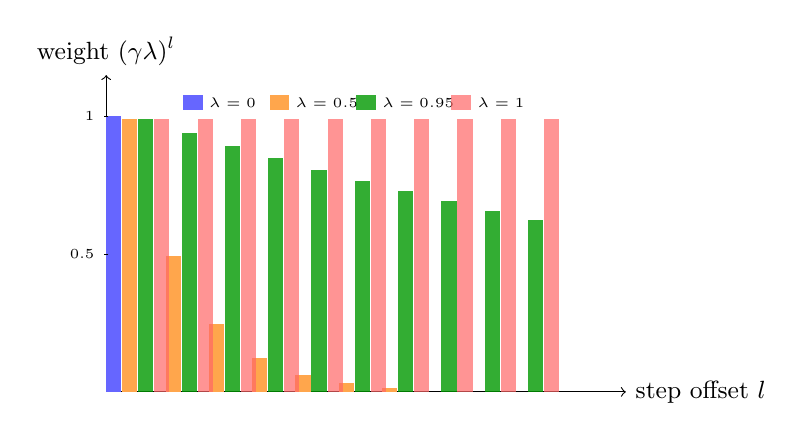
\begin{tikzpicture}[xscale=0.55, yscale=3.5]
  % Axes
  \draw[->] (0,0) -- (12,0) node[right, font=\small] {step offset $l$};
  \draw[->] (0,0) -- (0,1.15) node[above, font=\small] {weight $(\gamma\lambda)^l$};

  % lambda = 0: spike at l=0 only
  \fill[blue!60] (0,0) rectangle (0.35,1.0);

  % lambda = 0.5 bars
  \fill[orange!70] (0.37,0) rectangle (0.72,0.990);
  \fill[orange!70] (1.37,0) rectangle (1.72,0.495);
  \fill[orange!70] (2.37,0) rectangle (2.72,0.248);
  \fill[orange!70] (3.37,0) rectangle (3.72,0.124);
  \fill[orange!70] (4.37,0) rectangle (4.72,0.062);
  \fill[orange!70] (5.37,0) rectangle (5.72,0.031);
  \fill[orange!70] (6.37,0) rectangle (6.72,0.015);

  % lambda = 0.95 bars
  \fill[green!60!black,opacity=0.8] (0.74,0) rectangle (1.09,0.990);
  \fill[green!60!black,opacity=0.8] (1.74,0) rectangle (2.09,0.941);
  \fill[green!60!black,opacity=0.8] (2.74,0) rectangle (3.09,0.894);
  \fill[green!60!black,opacity=0.8] (3.74,0) rectangle (4.09,0.849);
  \fill[green!60!black,opacity=0.8] (4.74,0) rectangle (5.09,0.807);
  \fill[green!60!black,opacity=0.8] (5.74,0) rectangle (6.09,0.767);
  \fill[green!60!black,opacity=0.8] (6.74,0) rectangle (7.09,0.728);
  \fill[green!60!black,opacity=0.8] (7.74,0) rectangle (8.09,0.692);
  \fill[green!60!black,opacity=0.8] (8.74,0) rectangle (9.09,0.657);
  \fill[green!60!black,opacity=0.8] (9.74,0) rectangle (10.09,0.624);

  % lambda = 1 bars (uniform weight gamma^l ~ 0.99^l ~ constant for short ep)
  \fill[red!60,opacity=0.7] (1.11,0) rectangle (1.46,0.990);
  \fill[red!60,opacity=0.7] (2.11,0) rectangle (2.46,0.990);
  \fill[red!60,opacity=0.7] (3.11,0) rectangle (3.46,0.990);
  \fill[red!60,opacity=0.7] (4.11,0) rectangle (4.46,0.990);
  \fill[red!60,opacity=0.7] (5.11,0) rectangle (5.46,0.990);
  \fill[red!60,opacity=0.7] (6.11,0) rectangle (6.46,0.990);
  \fill[red!60,opacity=0.7] (7.11,0) rectangle (7.46,0.990);
  \fill[red!60,opacity=0.7] (8.11,0) rectangle (8.46,0.990);
  \fill[red!60,opacity=0.7] (9.11,0) rectangle (9.46,0.990);
  \fill[red!60,opacity=0.7] (10.11,0) rectangle (10.46,0.990);

  % y ticks
  \draw (0.05,1) -- (-0.05,1) node[left, font=\tiny] {1};
  \draw (0.05,0.5) -- (-0.05,0.5) node[left, font=\tiny] {0.5};

  % Legend inside
  \node[fill=blue!60, minimum width=0.25cm, minimum height=0.2cm,
        inner sep=0pt] at (2.0, 1.05) {};
  \node[right, font=\tiny] at (2.15, 1.05) {$\lambda=0$};
  \node[fill=orange!70, minimum width=0.25cm, minimum height=0.2cm,
        inner sep=0pt] at (4.0, 1.05) {};
  \node[right, font=\tiny] at (4.15, 1.05) {$\lambda=0.5$};
  \node[fill=green!60!black, minimum width=0.25cm, minimum height=0.2cm,
        inner sep=0pt, opacity=0.8] at (6.0, 1.05) {};
  \node[right, font=\tiny] at (6.15, 1.05) {$\lambda=0.95$};
  \node[fill=red!60, minimum width=0.25cm, minimum height=0.2cm,
        inner sep=0pt, opacity=0.7] at (8.2, 1.05) {};
  \node[right, font=\tiny] at (8.35, 1.05) {$\lambda=1$};

\end{tikzpicture}
\caption{Effective weights $(\gamma\lambda)^l$ on step-offset-$l$ TD errors
in GAE, for $\gamma = 0.99$ and four values of $\lambda$.  At $\lambda=0$
only the immediate TD error contributes; at $\lambda=1$ all steps receive
nearly uniform weight (decaying only by $\gamma^l \approx 1$).  Intermediate
$\lambda$ gives a soft exponential cutoff.}
\label{fig:gae-lambda}
\end{figure}

\subsection{The GAE Target for the Critic}

GAE also provides a natural target for training the critic.  Because
$\hat{A}_t^{\mathrm{GAE}} = \hat{V}_t - V_\phi(S_t)$, where
\begin{equation}
\label{eq:gae-vtarget}
\hat{V}_t = \hat{A}_t^{\mathrm{GAE}} + V_\phi(S_t),
\end{equation}
the critic can be trained by minimizing the mean-squared error
$\E[(V_\phi(S_t) - \hat{V}_t)^2]$ with $\hat{V}_t$ treated as a fixed
target.  This creates a consistent pair: the actor uses
$\hat{A}_t^{\mathrm{GAE}}$ for the policy gradient, and the critic uses
$\hat{V}_t$ as a regression target.

% -----------------------------------------------------------
\section{A2C and A3C}
\label{sec:a3c}
% -----------------------------------------------------------

\subsection{Parallelism as a Variance Reduction Tool}

One practical challenge with on-policy actor-critic algorithms is that
consecutive transitions $\{(S_t, A_t, R_{t+1}, S_{t+1})\}$ collected by a
single agent are highly \emph{correlated}: the agent follows a single
Markov chain, so nearby samples share similar states.  High correlation
inflates the effective variance of the gradient estimate even when the
per-sample variance is low.

Mnih et al.~(2016) proposed the \textbf{Asynchronous Advantage Actor-Critic}
(A3C)\index{A3C} as a solution.  The idea is to run multiple independent
\emph{worker} processes, each with its own copy of the environment and its
own local copy of the network parameters.  Workers generate experience
independently and asynchronously push gradient updates to a central
parameter server, which aggregates the updates.

\begin{definition}[A3C architecture]
\label{def:a3c}
\index{A3C}
In A3C, $K$ worker processes run in parallel.  Each worker $k$:
\begin{enumerate}[label=\arabic*., leftmargin=*]
  \item Copies global parameters $(\theta, \phi)$ to local copies
    $(\theta_k, \phi_k)$.
  \item Collects a short trajectory of $t_\mathrm{max}$ transitions using
    $\pi_{\theta_k}$.
  \item Computes actor and critic gradients using the advantage estimate
    $\hat{A}_t$ from~\eqref{eq:n-step-advantage}.
  \item Asynchronously applies gradients to the global $(\theta, \phi)$.
\end{enumerate}
\end{definition}

Because different workers typically find themselves in different states and
explore different parts of the state space simultaneously, their gradients
are nearly uncorrelated even without experience replay.  This decorrelation
is the key benefit of asynchronous parallelism.

\subsection{A2C: the Synchronous Variant}

\textbf{Advantage Actor-Critic} (A2C)\index{A2C} is the synchronous version
of A3C.  All $K$ workers collect a batch of transitions simultaneously, and
the parameter update is performed only after all workers have reported.
Because updates are synchronous, there is no inconsistency between the
parameters used to generate data and those being updated.

\begin{algorithm}[ht]
\caption{Advantage Actor-Critic (A2C)}
\label{alg:a2c}
\DontPrintSemicolon
\KwIn{$K$ parallel workers, rollout length $T_\mathrm{roll}$,
      discount $\gamma$, GAE parameter $\lambda$}
Initialize global $\theta, \phi$\;
\Repeat{convergence}{
  \For{each worker $k = 1, \ldots, K$ \emph{in parallel}}{
    Run $\pi_\theta$ for $T_\mathrm{roll}$ steps; collect
    $\{(S_t^k, A_t^k, R_{t+1}^k)\}_{t=0}^{T_\mathrm{roll}-1}$\;
    Compute $\hat{A}_t^k$ via GAE~\eqref{eq:gae-def}\;
    Compute $\hat{V}_t^k$ via~\eqref{eq:gae-vtarget}\;
  }
  Aggregate gradients across all workers\;
  Update $\theta$ using actor gradient
    $\frac{1}{KT_\mathrm{roll}}\sum_k\sum_t
     \hat{A}_t^k\,\nabla_\theta \log\pi_\theta(A_t^k|S_t^k)$\;
  Update $\phi$ by minimizing
    $\frac{1}{KT_\mathrm{roll}}\sum_k\sum_t
     (V_\phi(S_t^k) - \hat{V}_t^k)^2$\;
}
\end{algorithm}

In practice A2C achieves performance comparable to A3C and is easier to
implement reproducibly because the synchronous design eliminates race
conditions.  Modern deep RL pipelines almost universally use A2C-style
synchronous batching as the backbone, later enhanced with the trust-region
constraints developed in the next section.

% -----------------------------------------------------------
\section{Trust Region Methods}
\label{sec:trpo}
% -----------------------------------------------------------

\subsection{Off-Policy Reuse via Importance Sampling}

On-policy methods like A2C collect a batch of transitions and then discard
them immediately after a single gradient update.  This is wasteful: each
environment interaction is expensive (in simulation time, computation, or
real-world cost), but the on-policy constraint forces every sample to be
thrown away once the parameters change.

A natural remedy is importance sampling (introduced in Chapter~\ref{ch:mc}
in the context of off-policy Monte Carlo).  Suppose data was collected using
an \emph{old} policy $\pi_{\theta_\mathrm{old}}$ and we wish to evaluate or
optimize the \emph{new} policy $\pi_\theta$.  Define the per-step
\textbf{importance ratio}:\index{importance ratio}
\begin{equation}
\label{eq:importance-ratio}
r_t(\theta)
= \frac{\pi_\theta(A_t \mid S_t)}{\pi_{\theta_\mathrm{old}}(A_t \mid S_t)}.
\end{equation}
By standard importance sampling, the policy gradient
$\E_{\pi_\theta}[\nabla_\theta \log\pi_\theta(A|S)\,A^\pi(S,A)]$ can be
rewritten, under the approximation that the state distribution induced by
$\pi_\theta$ is close to that of $\pi_{\theta_\mathrm{old}}$, as
\begin{equation}
\label{eq:surrogate-obj}
L(\theta) = \E_{\pi_{\theta_\mathrm{old}}}\bigl[r_t(\theta)\,\hat{A}_t\bigr].
\end{equation}
The function $L(\theta)$ is called the \textbf{surrogate objective}.
\index{surrogate objective}
It can be optimized using data from $\pi_{\theta_\mathrm{old}}$, which
enables multiple gradient steps on the same batch.

\begin{proposition}[Surrogate gradient equals policy gradient at $\theta_\mathrm{old}$]
\label{prop:surrogate-gradient}
\begin{equation}
\label{eq:surrogate-gradient}
\nabla_\theta L(\theta)\big|_{\theta = \theta_\mathrm{old}}
= \nabla_\theta J(\theta)\big|_{\theta = \theta_\mathrm{old}}.
\end{equation}
\end{proposition}

\begin{proof}
At $\theta = \theta_\mathrm{old}$, $r_t(\theta) = 1$ for all transitions.
Differentiating $L(\theta) = \E[r_t(\theta)\,\hat{A}_t]$ gives
\[
\nabla_\theta L(\theta)\big|_{\theta_\mathrm{old}}
= \E\bigl[\nabla_\theta r_t(\theta)\big|_{\theta_\mathrm{old}}\cdot \hat{A}_t\bigr].
\]
Since $\nabla_\theta r_t(\theta) =
\frac{\nabla_\theta \pi_\theta(A_t|S_t)}{\pi_{\theta_\mathrm{old}}(A_t|S_t)}$,
at $\theta = \theta_\mathrm{old}$ this equals
$\nabla_\theta \log \pi_\theta(A_t|S_t)|_{\theta_\mathrm{old}}$,
giving the policy gradient.
\end{proof}

\subsection{The Danger of Large Updates}

Proposition~\ref{prop:surrogate-gradient} shows that the surrogate objective
is locally correct, but what happens when $\theta$ moves far from
$\theta_\mathrm{old}$?

\begin{proposition}[Monotone improvement bound]
\label{prop:monotone-improvement}
\index{trust region!monotone improvement bound}
There exists a constant $C > 0$ depending on $\gamma$ and
$\max_{s,a}|A^{\pi_\theta}(s,a)|$ such that
\begin{equation}
\label{eq:improvement-bound}
J(\theta) \geq L(\theta)
- C \cdot \max_s \KL{\pi_\theta(\cdot|s)}{\pi_{\theta_\mathrm{old}}(\cdot|s)}.
\end{equation}
\end{proposition}

The bound~\eqref{eq:improvement-bound}, due to Schulman et al.~(2015),
says that $J(\theta)$ is lower-bounded by $L(\theta)$ minus a term
proportional to the KL divergence of the new policy from the old one.
If the KL is small, the surrogate $L(\theta)$ is a reliable approximation
to $J(\theta)$, so maximizing $L$ guarantees improvement in $J$.  If the
KL is large, the bound is uninformative: the surrogate could rise while the
true objective falls.

This is the fundamental motivation for the trust region\index{trust region}
approach: we should only move $\theta$ within a region where the KL
divergence from $\theta_\mathrm{old}$ is small enough that
the surrogate is trustworthy.

\subsection{Trust Region Policy Optimization (TRPO)}

\textbf{Trust Region Policy Optimization} (TRPO)\index{TRPO},
introduced by Schulman et al.~(2015), solves the constrained optimization
problem:
\begin{equation}
\label{eq:trpo}
\max_\theta\; L(\theta)
\quad\text{subject to}\quad
\max_s\;\KL{\pi_\theta(\cdot|s)}{\pi_{\theta_\mathrm{old}}(\cdot|s)} \leq \delta,
\end{equation}
where $\delta > 0$ is a hyperparameter controlling the size of the trust
region.  In practice the maximum over states is replaced by an empirical
average.

Solving~\eqref{eq:trpo} requires computing the Fisher information matrix
(the Hessian of the KL constraint) and solving a constrained quadratic
programme.  This is done approximately via conjugate gradient with a line
search, but the procedure is computationally heavy: it requires multiple
Hessian-vector products per update, scaling poorly to networks with millions
of parameters.  TRPO is theoretically well-motivated but rarely used in
practice for large models.

PPO, developed next, provides a much simpler approximation to the same idea.

% -----------------------------------------------------------
\section{Proximal Policy Optimization}
\label{sec:ppo}
% -----------------------------------------------------------

\subsection{From Trust Regions to Clipping}

Proximal Policy Optimization (PPO)\index{PPO},
introduced by Schulman et al.~(2017), replaces the explicit KL constraint
of TRPO with a simple clipping operation on the importance ratio.
The intuition is that $r_t(\theta) = 1$ when $\theta = \theta_\mathrm{old}$,
and that allowing $r_t(\theta)$ to deviate far from 1 corresponds to a large
policy change.  PPO directly prevents large deviations by clipping $r_t$
to the interval $[1-\varepsilon, 1+\varepsilon]$ for a hyperparameter
$\varepsilon > 0$ (typically $\varepsilon \in [0.1, 0.3]$).

\begin{definition}[PPO clipped objective]
\label{def:ppo-clip}
\index{PPO!clipped objective}
The \textbf{PPO clipped surrogate objective} is
\begin{equation}
\label{eq:ppo-clip}
L^{\mathrm{CLIP}}(\theta)
= \E\!\left[\min\!\Bigl(
    r_t(\theta)\,\hat{A}_t,\;
    \operatorname{clip}\!\bigl(r_t(\theta),\,1-\varepsilon,\,1+\varepsilon\bigr)
    \,\hat{A}_t
  \Bigr)\right],
\end{equation}
where $\operatorname{clip}(x, a, b) = \max(a, \min(b, x))$.
\end{definition}

\subsection{Case Analysis of the Clipping Mechanism}

\begin{theorem}[Correctness of PPO clipping]
\label{thm:ppo-clip-cases}
\index{PPO!clipping cases}
For each transition, the clipped objective $L^{\mathrm{CLIP}}$
has the following properties:
\begin{enumerate}[label=(\roman*), leftmargin=*]
  \item If $\hat{A}_t > 0$: $L^{\mathrm{CLIP}}$ is non-decreasing in
    $r_t(\theta)$ for $r_t \leq 1+\varepsilon$, and constant for
    $r_t > 1+\varepsilon$.  The gradient is zero when $r_t > 1+\varepsilon$.
  \item If $\hat{A}_t < 0$: $L^{\mathrm{CLIP}}$ is non-increasing in
    $r_t(\theta)$ for $r_t \geq 1-\varepsilon$, and constant for
    $r_t < 1-\varepsilon$.  The gradient is zero when $r_t < 1-\varepsilon$.
  \item At $\theta = \theta_\mathrm{old}$ (so $r_t = 1 \in
    [1-\varepsilon, 1+\varepsilon]$), the gradient of $L^{\mathrm{CLIP}}$
    equals the policy gradient.
\end{enumerate}
\end{theorem}

\begin{proof}
Fix a transition and write $r = r_t(\theta)$, $A = \hat{A}_t$.
Let $f_1(r) = r A$ and $f_2(r) = \operatorname{clip}(r, 1-\varepsilon, 1+\varepsilon)\cdot A$.

\medskip
\textit{Case (i): $A > 0$.}
Then $f_1$ is strictly increasing in $r$.  For $r \leq 1+\varepsilon$,
the clip is inactive: $f_2(r) = rA = f_1(r)$.  For $r > 1+\varepsilon$,
$f_2(r) = (1+\varepsilon)A$, a constant.  So
\[
\min(f_1, f_2)
= \begin{cases} rA & r \leq 1+\varepsilon, \\ (1+\varepsilon)A & r > 1+\varepsilon.\end{cases}
\]
This is non-decreasing and its derivative with respect to $r$ is zero for
$r > 1+\varepsilon$.  No gradient incentive exists to increase the
probability of a good action beyond the $(1+\varepsilon)$ cap.

\medskip
\textit{Case (ii): $A < 0$.}
Then $f_1$ is strictly decreasing.  For $r \geq 1-\varepsilon$, $f_2(r) = rA = f_1(r)$.
For $r < 1-\varepsilon$, $f_2(r) = (1-\varepsilon)A$, a constant, and
$f_1(r) < f_2(r)$ since $A < 0$.  So $\min(f_1, f_2) = f_1(r) = rA$ for
$r < 1-\varepsilon$ (where $f_1 < f_2$) and $\min(f_1,f_2) = rA = f_2(r)$
for $r \in [1-\varepsilon, \infty)$.  Concretely,
\[
\min(f_1, f_2)
= \begin{cases} rA & r < 1-\varepsilon, \\ rA & r \geq 1-\varepsilon. \end{cases}
\]
Wait\,---\,let us be more careful.  For $A < 0$ and $r < 1-\varepsilon$:
$f_2(r) = (1-\varepsilon)A$ (constant, clipped from below), and
$f_1(r) = rA > (1-\varepsilon)A$ since $r < 1-\varepsilon$ and $A<0$.
So $f_1 > f_2$, thus $\min(f_1,f_2) = f_2 = (1-\varepsilon)A$, constant.
For $r \geq 1-\varepsilon$: clip is inactive, $f_2 = rA = f_1$,
so $\min = rA$.  Hence
\[
\min(f_1, f_2)
= \begin{cases} (1-\varepsilon)A & r < 1-\varepsilon, \\ rA & r \geq 1-\varepsilon.\end{cases}
\]
The gradient with respect to $r$ is zero for $r < 1-\varepsilon$:
there is no incentive to aggressively reduce the probability of a bad action
beyond the $(1-\varepsilon)$ floor.

\medskip
\textit{Case (iii):} At $r = 1 \in (1-\varepsilon, 1+\varepsilon)$ the clip
is inactive in both cases, so $L^{\mathrm{CLIP}} = \E[r_t(\theta)\hat{A}_t]
= L(\theta)$ in a neighbourhood of $\theta_\mathrm{old}$.
By Proposition~\ref{prop:surrogate-gradient}, $\nabla_\theta L^{\mathrm{CLIP}}
|_{\theta_\mathrm{old}} = \nabla_\theta J(\theta)|_{\theta_\mathrm{old}}$.
\end{proof}

The $\min$ operator in Definition~\ref{def:ppo-clip} is crucial: it makes
$L^{\mathrm{CLIP}}$ a \emph{pessimistic lower bound} on the surrogate
$r_t(\theta)\hat{A}_t$.  Figure~\ref{fig:ppo-clip} illustrates the two cases.

\begin{figure}[ht]
\centering
\begin{tikzpicture}[xscale=3.5, yscale=2.2]
  % Case 1: A > 0
  \begin{scope}[xshift=0cm]
    \def\eps{0.2}
    % Axes
    \draw[->] (0.5,0) -- (2.0,0) node[right, font=\small] {$r_t(\theta)$};
    \draw[->] (0.6,-0.1) -- (0.6,1.1)
              node[above, font=\small] {$L^{\mathrm{CLIP}}$};

    % Unclipped surrogate r*A (dashed)
    \draw[dashed, gray, thick] (0.65, 0.325) -- (1.9, 0.95);
    \node[gray, font=\tiny, right] at (1.85, 0.90) {$r\hat{A}$};

    % Clipped objective
    \draw[blue, very thick] (0.65, 0.325) -- (1.2, 0.6);
    \draw[blue, very thick] (1.2, 0.6) -- (1.9, 0.6);
    \fill[blue] (1.2, 0.6) circle (1.2pt);

    % Mark 1-eps, 1, 1+eps on x-axis
    \draw (0.8, 0.02) -- (0.8,-0.02) node[below, font=\tiny] {$1{-}\varepsilon$};
    \draw (1.0, 0.02) -- (1.0,-0.02) node[below, font=\tiny] {$1$};
    \draw (1.2, 0.02) -- (1.2,-0.02) node[below, font=\tiny] {$1{+}\varepsilon$};

    % Vertical dashed line at 1+eps
    \draw[dashed, gray!60] (1.2, 0) -- (1.2, 0.6);

    \node[font=\small, align=center] at (1.25, -0.28)
          {$\hat{A}_t > 0$: clip at $1+\varepsilon$};
  \end{scope}

  % Case 2: A < 0
  \begin{scope}[xshift=2.3cm]
    % Axes
    \draw[->] (0.5,0) -- (2.0,0) node[right, font=\small] {$r_t(\theta)$};
    \draw[->] (0.6,-0.85) -- (0.6,0.15)
              node[above, font=\small] {$L^{\mathrm{CLIP}}$};

    % Unclipped surrogate r*A (dashed, negative slope)
    \draw[dashed, gray, thick] (0.65, -0.065) -- (1.9, -0.57);
    \node[gray, font=\tiny, right] at (1.85, -0.55) {$r\hat{A}$};

    % Clipped objective
    \draw[red!80!black, very thick] (0.65, -0.325) -- (0.8, -0.325);
    \draw[red!80!black, very thick] (0.8, -0.325) -- (1.9, -0.57);
    \fill[red!80!black] (0.8, -0.325) circle (1.2pt);

    % Mark 1-eps, 1, 1+eps on x-axis
    \draw (0.8, 0.015) -- (0.8,-0.015) node[above, font=\tiny] {$1{-}\varepsilon$};
    \draw (1.0, 0.015) -- (1.0,-0.015) node[above, font=\tiny] {$1$};
    \draw (1.2, 0.015) -- (1.2,-0.015) node[above, font=\tiny] {$1{+}\varepsilon$};

    % Vertical dashed at 1-eps
    \draw[dashed, gray!60] (0.8, 0) -- (0.8, -0.325);

    \node[font=\small, align=center] at (1.25, -0.95)
          {$\hat{A}_t < 0$: clip at $1-\varepsilon$};
  \end{scope}
\end{tikzpicture}
\caption{The PPO clipping mechanism.  \emph{Left}: when $\hat{A}_t > 0$, the
objective is capped at $r_t = 1+\varepsilon$ (blue), preventing excessive
increases in action probability.  \emph{Right}: when $\hat{A}_t < 0$, the
objective is floored at $r_t = 1-\varepsilon$ (red), preventing excessive
decreases.  In both cases the $\min$ operator makes $L^{\mathrm{CLIP}}$ a
pessimistic lower bound on the unconstrained surrogate (dashed grey).}
\label{fig:ppo-clip}
\end{figure}

\subsection{Full PPO Objective}

In practice PPO optimizes a composite objective that combines the clipped
actor loss with a critic regression loss and an entropy bonus:
\begin{equation}
\label{eq:ppo-full}
\mathcal{L}(\theta, \phi)
= -L^{\mathrm{CLIP}}(\theta)
  + c_v\,\E\bigl[(V_\phi(S_t) - \hat{V}_t)^2\bigr]
  - c_H\,\E\bigl[-\log\pi_\theta(A_t \mid S_t)\bigr],
\end{equation}
where $\hat{V}_t$ is the GAE target~\eqref{eq:gae-vtarget}, $c_v > 0$
weights the value loss, and $c_H > 0$ weights the entropy bonus
$H(\pi_\theta({\cdot}|S_t))$.  The three terms serve distinct purposes:
\begin{description}[leftmargin=!, labelwidth=3.5cm]
  \item[$-L^{\mathrm{CLIP}}$] Maximizes the policy objective with a
    conservative trust-region constraint.
  \item[$c_v\,L^{\mathrm{VF}}$] Trains the critic to predict
    $V^{\pi_\theta}$, which is needed for accurate advantage estimation.
  \item[$-c_H\,H$] Adds an entropy bonus to discourage the policy from
    collapsing prematurely to a near-deterministic distribution,
    maintaining exploration throughout training.
\end{description}
When actor and critic share network layers, the entire
objective~\eqref{eq:ppo-full} is differentiated jointly.

\subsection{The PPO Algorithm}

\begin{algorithm}[ht]
\caption{Proximal Policy Optimization (PPO)}
\label{alg:ppo}
\DontPrintSemicolon
\KwIn{Rollout length $T$, workers $K$, epochs $K_e$,
      minibatch size $M$, clip $\varepsilon$, $\lambda$ for GAE}
Initialize $\theta$, $\phi$\;
\Repeat{convergence}{
  \tcp{Data collection}
  \For{each of $K$ workers in parallel}{
    Run $\pi_\theta$ for $T$ steps; store
    $\{S_t, A_t, R_{t+1}, S_{t+1}\}$\;
    Compute $\hat{A}_t^{\mathrm{GAE}}$ via~\eqref{eq:gae-def}
    and $\hat{V}_t$ via~\eqref{eq:gae-vtarget}\;
  }
  Normalize advantages: $\hat{A}_t \leftarrow
    (\hat{A}_t - \bar{A})/\hat{\sigma}_A$ across all workers\;
  Fix $\theta_\mathrm{old} \leftarrow \theta$\;
  \tcp{Multiple optimization epochs on collected data}
  \For{epoch $= 1, \ldots, K_e$}{
    \For{each minibatch $\mathcal{B}$ of size $M$}{
      Compute $r_t(\theta) = \pi_\theta(A_t|S_t)/\pi_{\theta_\mathrm{old}}(A_t|S_t)$
      for each $(S_t, A_t) \in \mathcal{B}$\;
      Compute $\mathcal{L}(\theta,\phi)$ via~\eqref{eq:ppo-full}\;
      Update $\theta, \phi$ by one step of Adam\;
    }
  }
}
\end{algorithm}

Several design choices in Algorithm~\ref{alg:ppo} deserve comment.

\begin{remark}[Advantage normalization]
Subtracting the batch mean and dividing by the batch standard deviation
(step ``Normalize advantages'') is a standard engineering practice.
It keeps the magnitude of the gradient roughly constant across episodes
regardless of the reward scale, which reduces sensitivity to the learning
rate and stabilizes training.  It introduces a mild bias because the
normalization changes the relative weighting of transitions, but this is
empirically beneficial.
\end{remark}

\begin{remark}[Multiple epochs]
PPO reuses each batch for $K_e$ gradient steps.  This substantially
improves sample efficiency compared with pure on-policy methods (where
data is discarded after one gradient step), while the clipping ensures
that the policy does not drift too far from the data-collection policy
within a single batch.  Typical values are $K_e \in [3, 10]$.
\end{remark}

\begin{example}[PPO on a simple MDP]
\label{ex:ppo-numeric}
Consider a three-state chain MDP with states $\{s_1, s_2, s_3\}$ where
$s_3$ is terminal.  The agent has two actions (left/right).  Suppose at
the current iteration:
\begin{itemize}[leftmargin=*]
  \item $\hat{A}_t = 0.8$ (the taken action was significantly above average).
  \item $r_t(\theta) = 1.35$ after a gradient step (the new policy assigns
    $35\%$ more probability to this action than the old policy did).
  \item $\varepsilon = 0.2$.
\end{itemize}
Without clipping, the contribution to $L$ would be $1.35 \times 0.8 = 1.08$.
With clipping, $r_t$ is capped at $1+\varepsilon = 1.2$, giving
$1.2 \times 0.8 = 0.96$.  Since $0.96 < 1.08$, the $\min$ selects $0.96$.
The gradient of $L^{\mathrm{CLIP}}$ with respect to $\theta$ is zero for this
sample because $r_t > 1+\varepsilon$: the policy has already moved far enough
in the direction of increasing this action's probability, and PPO provides
no additional gradient to push it further.\qed
\end{example}

% -----------------------------------------------------------
\section{PPO for Language Models}
\label{sec:ppo-llm}
% -----------------------------------------------------------

\subsection{Language Models as RL Policies}

The application of PPO to the fine-tuning of large language models (LLMs)
via human feedback\,---\,commonly called
RLHF\index{RLHF}\index{Reinforcement Learning from Human Feedback|see{RLHF}}---has
become one of the most practically important uses of reinforcement learning.
Chapter~\ref{ch:lm-post-training} studies language models as RL agents in detail;
here we focus specifically on the PPO component of the RLHF pipeline.

A language model $\pi_\theta$ defines an autoregressive policy over tokens.
Given a prompt $x = (x_1, \ldots, x_m)$, the model generates a response
$y = (y_1, \ldots, y_T)$ one token at a time:
\begin{equation}
\label{eq:lm-policy}
\pi_\theta(y \mid x)
= \prod_{t=1}^T \pi_\theta(y_t \mid x,\, y_1, \ldots, y_{t-1}).
\end{equation}
This maps to an MDP where the state at step $t$ is
$S_t = (x, y_1, \ldots, y_{t-1})$, the action is the next token
$A_t = y_t \in \mathcal{V}$ (the vocabulary), and the episode terminates
when an end-of-sequence token is generated.  The action space has size
$|\mathcal{V}| \in [32{,}000,\; 128{,}000]$\,---\,far larger than classical
RL benchmarks\,---\,making value-based methods impractical and policy-based
methods like PPO natural.

\subsection{Reward Modeling and the KL Penalty}

In RLHF, the reward signal comes from a separately trained
\textbf{reward model}\index{reward model} $r_\psi(x, y)$ that was fitted
to human preference comparisons.  In the simplest setting, a scalar reward
is emitted only at the end of the episode:
$R_t = 0$ for $t < T$ and $R_T = r_\psi(x, y)$.

Without further regularization, however, the policy rapidly learns to
exploit the reward model\,---\,a phenomenon called
\textbf{reward hacking}\index{reward hacking}.  The policy may produce
outputs that score highly under $r_\psi$ but diverge from coherent, safe,
and factually accurate language.  The standard remedy is a per-token
KL-divergence penalty relative to the
\emph{reference policy}\index{reference policy} $\pi_{\mathrm{ref}}$
(typically the supervised fine-tuned model before RL training):
\begin{equation}
\label{eq:rlhf-reward}
\tilde{R}_t(x, y)
=
\begin{cases}
r_\psi(x, y)
  - \beta\,\log\dfrac{\pi_\theta(y_T \mid x, y_{<T})}
                      {\pi_{\mathrm{ref}}(y_T \mid x, y_{<T})},
& t = T, \\[8pt]
- \beta\,\log\dfrac{\pi_\theta(y_t \mid x, y_{<t})}
                    {\pi_{\mathrm{ref}}(y_t \mid x, y_{<t})},
& t < T,
\end{cases}
\end{equation}
where $\beta > 0$ controls the strength of the KL penalty.

\begin{proposition}[RLHF total reward]
\label{prop:rlhf-kl}
The sum of adjusted per-step rewards satisfies
\begin{equation}
\label{eq:rlhf-total}
\sum_{t=1}^T \tilde{R}_t
= r_\psi(x, y)
  - \beta\,\KL{\pi_\theta(\cdot \mid x)}{\pi_{\mathrm{ref}}(\cdot \mid x)},
\end{equation}
where the KL divergence is computed over the joint sequence distribution.
\end{proposition}

\begin{proof}
Summing~\eqref{eq:rlhf-reward} over $t = 1, \ldots, T$,
\[
\sum_{t=1}^T \tilde{R}_t
= r_\psi(x,y)
  - \beta\sum_{t=1}^T
    \log\frac{\pi_\theta(y_t \mid x, y_{<t})}
             {\pi_{\mathrm{ref}}(y_t \mid x, y_{<t})}.
\]
The KL divergence between two autoregressive distributions
$\pi_\theta(\cdot|x)$ and $\pi_{\mathrm{ref}}(\cdot|x)$ factors as
\[
\KL{\pi_\theta(\cdot|x)}{\pi_{\mathrm{ref}}(\cdot|x)}
= \E_{y \sim \pi_\theta}\!\left[
  \sum_{t=1}^T \log\frac{\pi_\theta(y_t|x,y_{<t})}
                         {\pi_{\mathrm{ref}}(y_t|x,y_{<t})}
\right],
\]
so the per-sample sum $\sum_t \log[\pi_\theta/\pi_{\mathrm{ref}}]$ is an
unbiased Monte Carlo estimate of the KL.  Substituting gives~\eqref{eq:rlhf-total}.
\end{proof}

Proposition~\ref{prop:rlhf-kl} reveals the objective that RLHF implicitly
optimizes: maximize reward model score minus a KL-weighted penalty for
diverging from the reference policy.  As $\beta \to 0$, the penalty
vanishes and the policy can drift arbitrarily far from $\pi_{\mathrm{ref}}$,
risking reward hacking.  As $\beta \to \infty$, the optimal policy is
$\pi_{\mathrm{ref}}$ itself and no reinforcement learning occurs.

\subsection{The Four-Model RLHF Architecture}

A standard PPO-RLHF training run maintains four neural network models
simultaneously:

\begin{description}[leftmargin=!, labelwidth=3.5cm]
  \item[Actor $\pi_\theta$] The policy being trained.  Its parameters are
    updated at every PPO iteration.
  \item[Critic $V_\phi$] A value head\,---\,typically a single linear layer
    applied to the final hidden state of the last token\,---\,that
    estimates the expected cumulative adjusted reward from state $S_t$.
  \item[Reference model $\pi_{\mathrm{ref}}$] A frozen copy of the
    supervised fine-tuned model, used only to compute the KL penalty
    in~\eqref{eq:rlhf-reward}.
  \item[Reward model $r_\psi$] A frozen model (usually the same
    architecture as the actor, with an added scalar head) trained on
    human preference data to output a scalar quality score.
\end{description}

The advantages $\hat{A}_t$ are computed via GAE applied to the adjusted
rewards $\tilde{R}_t$ from~\eqref{eq:rlhf-reward}, and the PPO clipped
objective~\eqref{eq:ppo-clip} is applied with the vocabulary-level
importance ratios $r_t(\theta) = \pi_\theta(y_t|x,y_{<t}) /
\pi_{\theta_\mathrm{old}}(y_t|x,y_{<t})$.

\begin{example}[PPO-RLHF on a question-answering task]
\label{ex:ppo-rlhf}
Suppose the prompt is ``Explain Fermat's Last Theorem.'' and the policy
generates a 120-token response $y$.  The reward model scores the full
response: $r_\psi(x,y) = 0.78$.  At each token step $t < 120$, the
per-token log-ratio $\log[\pi_\theta(y_t|x,y_{<t})/\pi_{\mathrm{ref}}(y_t|x,y_{<t})]$
is computed; if the policy has drifted modestly from the reference, each
term might be around $0.01$, contributing a cumulative KL penalty of
$\beta \times 0.01 \times 120 = 1.2\beta$.  With $\beta = 0.05$, the
total adjusted reward is $0.78 - 0.06 = 0.72$.

The critic $V_\phi(S_t)$ predicts the expected total adjusted reward from
the partial sequence seen so far.  After each token is generated,
$\delta_t = \tilde{R}_t + \gamma V_\phi(S_{t+1}) - V_\phi(S_t)$ is computed,
and GAE aggregates these errors into per-token advantage estimates.
A token such as ``Wiles'' (as in Andrew Wiles) that is both relevant and
specific may push the critic's prediction upward, yielding a positive
advantage that increases the probability of this token in future PPO
updates.\qed
\end{example}

\subsection{Practical Considerations}

The following guidelines distill empirical best practices from the RLHF
literature (Ouyang et al.\ 2022, Bai et al.\ 2022, Ziegler et al.\ 2019).

\paragraph{KL monitoring and control.}
Track the running average of $\KL{\pi_\theta}{\pi_{\mathrm{ref}}}$ across
prompt batches.  A rapid increase signals that the policy is diverging from
the reference model.  If the KL exceeds a preset threshold (e.g.\ 10~nats),
either increase $\beta$, reduce the learning rate, or halt training and
diagnose the reward model.

\paragraph{Advantage normalization.}
Normalize $\hat{A}_t$ to zero mean and unit variance across the minibatch
before computing the clipped objective.  For language generation, episodes
(responses) have varying lengths; normalization prevents long sequences
from dominating gradient updates purely because they accumulate more per-step
terms.

\paragraph{Critic initialization.}
Initialize the value head on top of the same pre-trained backbone as the
actor.  Starting from a randomly initialized critic produces wildly
inaccurate advantage estimates in early training, destabilizing the actor
before it has learned anything useful.

\paragraph{Epoch count per batch.}
Use $K_e \in [1, 4]$ optimization epochs per data batch for RLHF, versus
$K_e \in [4, 10]$ for classical RL environments.  Because the reward model
can be exploited (unlike a true environment), too many epochs on the same
batch encourage the actor to overfit to the reward model signal,
accelerating reward hacking.

\paragraph{Reward hacking detection.}
Periodically evaluate the trained policy on held-out prompts judged by
humans (or by a separate, independent evaluator).  If the reward model
score continues rising while human judgments plateau or decline, reward
hacking is occurring.  Mitigations include refreshing the reward model with
additional preference data, increasing $\beta$, or incorporating a
supervised fine-tuning loss alongside the PPO objective.

% -----------------------------------------------------------
\section{Convergence and Practical Considerations}
\label{sec:ac-convergence}
% -----------------------------------------------------------

\subsection{Convergence Properties}

The convergence theory for actor-critic methods is substantially more complex
than for pure TD or pure policy gradient methods, because both components
are being updated simultaneously and their objectives interact.

For the \emph{linear} function approximation case with a fixed policy, the
TD(0) critic converges to the solution of the projected Bellman equation,
as established in Chapter~\ref{ch:td}.  When the actor is also updated,
convergence requires \textbf{two-timescale stochastic approximation}: the
critic's step size $\alpha_\phi$ must decrease faster than the actor's
$\alpha_\theta$, ensuring the critic tracks $V^{\pi_\theta}$ faster than
$\pi_\theta$ changes.

\begin{theorem}[Two-timescale convergence, sketch]
\label{thm:two-timescale}
\index{actor-critic!two-timescale convergence}
Under the following conditions:
\begin{enumerate}[label=(\roman*), leftmargin=*]
  \item linear function approximation for the critic,
  \item Robbins-Monro step sizes satisfying
    $\sum_t \alpha_\phi(t) = \infty$, $\sum_t \alpha_\phi(t)^2 < \infty$,
    and $\alpha_\theta(t) / \alpha_\phi(t) \to 0$,
  \item the policy gradient ODE has a unique globally attracting equilibrium
    (or, more generally, the iterates remain bounded),
\end{enumerate}
the actor-critic algorithm converges almost surely to a stationary point of
the objective $J(\theta)$.
\end{theorem}

For \emph{nonlinear} function approximation (neural networks), no
comparably clean theory exists.  In practice, the actor and critic are
updated with the same optimizer (e.g.\ Adam) and the same or similar
learning rates, which violates the two-timescale requirement.  Yet PPO is
empirically stable across a wide range of tasks, suggesting that the
neural networks act as their own effective regularizers.

\subsection{Comparison of Policy Gradient Algorithms}

Table~\ref{tab:pg-comparison} summarizes the key properties of the policy
gradient family discussed in Chapters~\ref{ch:pg} and~\ref{ch:actor-critic}.

\begin{table}[ht]
\centering
\caption{Comparison of policy gradient algorithms.
``On-policy'' means each data sample is used for at most one gradient update.}
\label{tab:pg-comparison}
\begin{tabular}{@{}lcccc@{}}
\toprule
Algorithm & Baseline & Online? & Multiple epochs? & Trust region? \\
\midrule
REINFORCE               & None / constant  & No  & No  & No  \\
REINFORCE + baseline    & $V_\phi(s)$      & No  & No  & No  \\
One-step AC             & TD(0) critic     & Yes & No  & No  \\
A2C / A3C               & GAE critic       & Yes & No  & No  \\
TRPO                    & GAE critic       & Yes & No  & KL constraint \\
PPO                     & GAE critic       & Yes & Yes & Clip $\varepsilon$ \\
\bottomrule
\end{tabular}
\end{table}

\subsection{Hyperparameter Sensitivity and Implementation Tips}

PPO is notably robust to hyperparameter choices relative to TRPO, which
requires careful tuning of the conjugate gradient step count and
line-search parameters.  Nevertheless, the following guidelines are helpful
in practice.

\begin{description}[leftmargin=!, labelwidth=3.5cm]
  \item[Clip parameter $\varepsilon$] Typical values are $0.1$ to $0.3$.
    Smaller $\varepsilon$ gives more conservative updates and is safer for
    fine-tuning large pretrained models.  $\varepsilon = 0.2$ is the most
    common default.
  \item[GAE $\lambda$] Values $0.90$--$0.97$ work well across most tasks.
    Longer episodes warrant larger $\lambda$ (to capture long-range credit).
  \item[Value coefficient $c_v$] Typically $0.5$; can be reduced if the
    value network is separately optimized or if gradient magnitudes are
    already well-matched.
  \item[Entropy coefficient $c_H$] Start with $0.01$; increase if the
    policy collapses prematurely to a near-deterministic distribution.
  \item[Epochs per batch $K_e$] Values $4$--$8$ for continuous control;
    $1$--$4$ for RLHF.  Monitor the KL between $\pi_\theta$ and
    $\pi_{\theta_\mathrm{old}}$ and stop epochs early if KL exceeds
    $\sim 1.5\varepsilon$.
  \item[Batch and minibatch size] Larger batches reduce gradient noise but
    require more memory.  A rollout of $2048$ steps with minibatch size $64$
    is a common starting point for continuous control.
  \item[Learning rate] $3 \times 10^{-4}$ with Adam is a robust default.
    Linear or cosine decay schedules often help for fine-tuning.
  \item[Observation normalization] Normalize observations to zero mean and
    unit variance (with running statistics) and clip rewards to a fixed
    range (e.g.\ $[-5, 5]$) to prevent the critic from being overwhelmed
    by outlier rewards.
\end{description}

% -----------------------------------------------------------
\section*{Exercises}
\addcontentsline{toc}{section}{Exercises}
\label{sec:ch9-exercises}
% -----------------------------------------------------------

\begin{exercise}
\label{ex:advantage-computation}
Consider an MDP with three actions available in state $s$.
Suppose $Q^{\pi}(s, a_1) = 5$, $Q^{\pi}(s, a_2) = 8$, $Q^{\pi}(s, a_3) = 2$,
and the policy assigns probabilities $\pi(a_1|s) = 0.5$, $\pi(a_2|s) = 0.3$,
$\pi(a_3|s) = 0.2$.
\begin{enumerate}[label=(\alph*)]
  \item Compute $V^\pi(s)$ and the advantage $A^\pi(s, a_i)$ for each action.
  \item Verify that $\E_{A \sim \pi(\cdot|s)}[A^\pi(s,A)] = 0$.
  \item A gradient step increases $\pi(a_2|s)$.  Explain why using
    $A^\pi(s,a_2) = 2$ (rather than $Q^\pi(s,a_2) = 8$) as the gradient
    weight leads to a smaller but more informative update.
\end{enumerate}
\end{exercise}

\begin{exercise}
\label{ex:td-advantage-numeric}
A critic with $V_\phi = V^{\pi_\theta}$ observes a transition
$(S_t, A_t, R_{t+1}, S_{t+1})$ with $R_{t+1} = 2$, $\gamma = 0.9$,
$V^\pi(S_t) = 3$, $V^\pi(S_{t+1}) = 4$.
\begin{enumerate}[label=(\alph*)]
  \item Compute the TD error $\delta_t$.
  \item Is the action $A_t$ above or below average in state $S_t$?
    Justify using the sign of $\delta_t$.
  \item After one actor update with step size $\alpha_\theta = 0.01$
    and $\gamma^t = 1$, by how much does
    $\log \pi_\theta(A_t|S_t)$ change?
\end{enumerate}
\end{exercise}

\begin{exercise}
\label{ex:gae-derivation}
Let $T = 4$ (steps $t = 0,1,2,3$, terminal at $t=4$) with TD errors
$\delta_0 = 0.4$, $\delta_1 = -0.2$, $\delta_2 = 0.6$, $\delta_3 = 0.1$.
Take $\gamma = 1$ and $\lambda = 0.8$.
\begin{enumerate}[label=(\alph*)]
  \item Compute $\hat{A}_0^{\mathrm{GAE}}$ using Definition~\ref{def:gae}.
  \item Verify that your answer matches the formula from
    Proposition~\ref{prop:gae-nstep} by computing the weighted mixture of
    $n$-step advantages $\hat{A}_0^{(n)}$ for $n = 1, 2, 3, 4$.
  \item Compute $\hat{A}_0^{\mathrm{GAE}}$ for $\lambda = 0$ and
    $\lambda = 1$ and interpret the results.
\end{enumerate}
\end{exercise}

\begin{exercise}
\label{ex:ppo-clip-numerical}
Consider the PPO clipped objective with $\varepsilon = 0.2$.
\begin{enumerate}[label=(\alph*)]
  \item Compute $L^{\mathrm{CLIP}}$ contributions for the following
    three transitions and indicate whether the clip is active:
    \begin{enumerate}[label=(\roman*)]
      \item $\hat{A}_t = 1.5$, $r_t(\theta) = 0.8$.
      \item $\hat{A}_t = 1.5$, $r_t(\theta) = 1.3$.
      \item $\hat{A}_t = -0.5$, $r_t(\theta) = 0.75$.
    \end{enumerate}
  \item For case (ii) above, explain why the gradient of
    $L^{\mathrm{CLIP}}$ with respect to $\theta$ is zero even though
    $\hat{A}_t > 0$ and the action should be encouraged.
    Why is this conservative behaviour desirable?
\end{enumerate}
\end{exercise}

\begin{exercise}
\label{ex:surrogate-gradient-proof}
This exercise works through the surrogate gradient
(Proposition~\ref{prop:surrogate-gradient}) in detail.
\begin{enumerate}[label=(\alph*)]
  \item Show that $r_t(\theta)|_{\theta=\theta_\mathrm{old}} = 1$ for all
    transitions.
  \item Write $\nabla_\theta r_t(\theta)$ in terms of the policy and
    show it equals $r_t(\theta)\,\nabla_\theta \log\pi_\theta(A_t|S_t)$.
  \item Conclude that $\nabla_\theta L(\theta)|_{\theta_\mathrm{old}}
    = \E[\nabla_\theta\log\pi_{\theta_\mathrm{old}}(A_t|S_t)\,\hat{A}_t]$
    and explain why this is exactly the policy gradient.
\end{enumerate}
\end{exercise}

\begin{exercise}
\label{ex:rlhf-kl}
In the RLHF adjusted reward~\eqref{eq:rlhf-reward}, set $\gamma = 1$.
\begin{enumerate}[label=(\alph*)]
  \item Prove Proposition~\ref{prop:rlhf-kl} from first principles,
    using only the chain rule of KL divergence for autoregressive models.
  \item Show that the optimal policy for the objective
    $\max_\pi \E[r_\psi(x,y)] - \beta\,\KL{\pi(\cdot|x)}{\pi_{\mathrm{ref}}(\cdot|x)}$
    is $\pi^*(y|x) \propto \pi_{\mathrm{ref}}(y|x)\,e^{r_\psi(x,y)/\beta}$.
  \item Interpret the optimal policy: what happens as $\beta \to 0$?
    As $\beta \to \infty$?  What does this imply for the choice of $\beta$
    in practice?
\end{enumerate}
\end{exercise}

\begin{exercise}
\label{ex:ac-comparison-table}
Fill in the following comparison table for three algorithms:
REINFORCE with baseline, one-step actor-critic, and PPO.
For each row, answer ``yes'' / ``no'' or give a brief phrase.

\begin{center}
\begin{tabular}{@{}lccc@{}}
\toprule
Property & REINFORCE+BL & One-step AC & PPO \\
\midrule
Requires full episode?         & & & \\
Data reuse across updates?     & & & \\
Advantage estimator            & & & \\
Online (step-by-step) updates? & & & \\
Trust-region constraint?       & & & \\
\bottomrule
\end{tabular}
\end{center}
\end{exercise}

\begin{exercise}
\label{ex:gae-bias-variance}
Explain, using the decomposition in Proposition~\ref{prop:gae-nstep},
why GAE with $\lambda < 1$ has lower variance than the Monte Carlo advantage
estimate $G_t - V_\phi(S_t)$, but introduces bias.
\begin{enumerate}[label=(\alph*)]
  \item Identify the source of variance in the Monte Carlo estimate
    (Hint: count the number of independent random variables in $G_t$).
  \item Identify the source of bias in the GAE estimate for $\lambda < 1$
    (Hint: consider what happens when $V_\phi \neq V^\pi$).
  \item State informally why $\lambda \approx 0.95$ is a sensible
    default for episodes of length $\sim 1000$.
\end{enumerate}
\end{exercise}

\begin{exercise}
\label{ex:two-timescale}
The two-timescale convergence result (Theorem~\ref{thm:two-timescale})
requires $\alpha_\theta(t)/\alpha_\phi(t) \to 0$.
\begin{enumerate}[label=(\alph*)]
  \item Explain intuitively why the critic must learn faster than the actor.
    What goes wrong if the actor updates are as fast as the critic's?
  \item Propose a concrete pair of step-size sequences
    $\alpha_\phi(t) = 1/(t+1)$ and $\alpha_\theta(t)$ satisfying the
    two-timescale condition.
  \item In modern PPO implementations with Adam, both actor and critic use
    the same optimizer and learning rate.  What practical mechanism replaces
    the two-timescale requirement?
\end{enumerate}
\end{exercise}

\begin{exercise}[Challenge]
\label{ex:trpo-ppo-connection}
This exercise establishes a precise connection between TRPO and PPO.
\begin{enumerate}[label=(\alph*)]
  \item Show that the TRPO constraint
    $\KL{\pi_\theta}{\pi_{\theta_\mathrm{old}}} \leq \delta$
    implies $|r_t(\theta) - 1| \leq \sqrt{2\delta}$ for any single
    action-state pair, using Pinsker's inequality
    $\|\pi - q\|_1 \leq \sqrt{2\,\KL{\pi}{q}}$.
  \item Using part (a), argue that the PPO clip at $\varepsilon$ is
    a first-order approximation to the TRPO KL constraint with
    $\delta \approx \varepsilon^2/2$.
  \item Discuss one advantage and one disadvantage of PPO's approximation
    relative to exact TRPO.
\end{enumerate}
\end{exercise}
